% ============================================================
% setquant paper - compile on Overleaf (pdfLaTeX + BibTeX)
% Tables/figure are AUTO-GENERATED: python scripts/make_paper_assets.py
% %% TODO ... = จุดที่ควรเขียนใหม่ด้วยเสียงของตัวเองก่อนส่ง
% ============================================================
\documentclass[11pt]{article}
\usepackage[margin=1in]{geometry}
\usepackage{amsmath}
\usepackage{booktabs}
\usepackage{graphicx}
\usepackage{natbib}
\usepackage{caption}
\usepackage[colorlinks=true, allcolors=blue!40!black]{hyperref}

\title{Does Cross-Sectional Momentum Survive Transaction Costs in Thai Equities?\\
\large Evidence from a Survivorship-Bias-Controlled SET100 Sample, 2016--2026}
\author{[Your name]\thanks{Independent research project. Code and full experiment
log: \url{https://github.com/satangtecha/setquant}. All backtests, data pipelines
and this document are reproducible from the repository.}}
\date{July 2026}

\begin{document}
\maketitle

\begin{abstract}
%% TODO: ปรับ abstract ให้เป็นเสียงตัวเองหลังเนื้อหานิ่งแล้ว (เขียนท้ายสุด)
I test whether the cross-sectional momentum effect, one of the most robust
anomalies in global equity markets, survives realistic transaction costs in
Thailand. Using a point-in-time SET100 universe hand-assembled from the Stock
Exchange of Thailand's official semi-annual constituent lists (22 periods,
191 distinct members, 2016--2026), I form monthly-rebalanced, equal-weighted
portfolios of the top decile of stocks ranked by 12-1 momentum. Over
114 months, the strategy earns 4.90\% per year net of a 0.25\%-per-side cost
assumption, against 0.28\% for an equal-weight benchmark of the same
point-in-time universe --- an active return of 3.73\% per year. The point
estimate is economically meaningful and survives conservative cost
assumptions, but is not statistically significant ($t = 0.98$); the
top-minus-bottom decile spread earns 8.49\% per year ($t = 1.32$).
Performance is concentrated in 2020--2022. I document the remaining data
limitations --- notably thirteen delisted index members with irrecoverable
price history --- and argue the residual bias modestly flatters the result.
The hypothesis, registered before estimation, is therefore neither confirmed
nor rejected: a realistic outcome for a single decade of data in a small
market.
\end{abstract}

\section{Introduction}

%% TODO: ย่อหน้าแรกควรเป็นของคุณเองมากที่สุด — ทำไมสนใจคำถามนี้
Momentum --- the tendency of stocks that performed well over the past year to
keep outperforming over the next month --- is among the most widely
documented return anomalies. \citet{jegadeesh1993returns} established the
effect in US equities; \citet{asness2013value} found it in every major asset
class; \citet{rouwenhorst1999local} showed it exists in emerging markets;
\citet{fama2012size} confirmed it in international portfolios. The open
question for a practitioner is never whether momentum existed in a
frictionless backtest, but whether it survives the real world: transaction
costs, index membership churn, delistings, and the temptation to keep tuning
parameters until something looks good.

This paper asks that question for the Thai stock market, which is a useful
laboratory for three reasons. First, it is under-studied relative to US and
pan-Asian samples, and the few available studies rarely control for
survivorship bias explicitly. Second, it is a market where realistic retail
execution costs are non-trivial and observable. Third, the decade
2016--2026 includes a full cycle of regimes: a sideways grind, the COVID
crash, a violent recovery, and a prolonged bear market --- a demanding
sample for any trend-based strategy.

Three design choices distinguish this study from a typical hobbyist
backtest. First, the investable universe at every formation date is the
actual SET100 membership on that date, transcribed from the Stock Exchange
of Thailand's official semi-annual constituent announcements, so stocks that
later collapsed or delisted are included while they were members. Second,
the hypothesis --- \emph{the top momentum decile of SET100 members,
rebalanced monthly, beats an equal-weight benchmark of the same universe
after realistic costs} --- was registered before any backtest was run, and
every experiment executed against the data is recorded in a public log
(Appendix~\ref{app:registry}); there is no hidden search over parameters.
Third, the backtest engine's two core correctness properties, point-in-time
membership and the absence of look-ahead, are enforced by unit tests that
construct deliberate traps (a non-member with an enormous signal; a stock
with an enormous future return) and assert the engine cannot see them.

%% TODO: สรุปผลหนึ่งย่อหน้า + roadmap ของ paper

\section{Data and universe construction}
\label{sec:data}

\subsection{Point-in-time index membership}
The universe is rebuilt from the SET's official ``SET50 and SET100 Index
Constituents'' documents, published for every half-year since 2005 and
available to registered SET members. I transcribe the 22 semi-annual lists
covering January 2016 through December 2026 with an automated PDF parser
that enforces two validators before accepting a list: each document must
contain exactly the row numbers 1--100, and the extracted symbols must be
strictly alphabetical --- an ordering the documents themselves guarantee
(``Rank by alphabet''). Documents revised mid-period (mergers,
restructurings) supersede the original for the whole period. The resulting
membership table contains 2{,}200 stock-period rows and 191 distinct
symbols; between 3 and 13 names change at each semi-annual revision.

A backtest at formation date $t$ sees exactly the stocks that were members
on $t$. Using today's membership for the past would exclude every stock
that has since left the index --- including all delistings --- and is the
canonical source of survivorship bias in retail backtests.

\subsection{Price data, renames, and silent gaps}
Daily prices come from Yahoo Finance (\texttt{.BK} tickers), stored
unmodified in a bronze layer and cleaned into a silver layer. Seven
corporate renames and restructurings (e.g.\ TMB$\to$TTB, TICON$\to$FPT,
LHBANK$\to$LHFG) are resolved through an explicit alias table; without it,
those stocks would silently vanish from the sample. A coverage check
compares each symbol's first data date against its first membership date
and flags every shortfall. Three classes emerge: benign IPO timing (e.g.\
AWC, +101 days), restructuring gaps where a ``new'' listed entity carries
no pre-restructuring history (SCB after the SCBX conversion, +2{,}301 days;
GULF after the INTUCH amalgamation, +2{,}284 days), and thirteen former
members --- BSRC, DTAC, EARTH, ESSO, GL, GLOW, GOLD, IFEC, INTUCH, KEX,
ROBINS, SABUY, STARK --- whose history is entirely absent from the vendor.
The full flagged list is reproduced in Appendix~\ref{app:gaps}.

\subsection{Adjusted prices and quality control}
Returns are computed from the vendor's dividend- and split-adjusted close.
As a cross-check, I independently reconstruct adjusted prices from the
vendor's raw dividend and split events; the two series agree to within
$10^{-7}$ for 159 of 171 downloadable names, but disagree badly (median
relative difference 9\%--1{,}100\%) for about a dozen --- evidence that the
vendor's \emph{event feed} misses several Thai par-value changes and splits
even though its adjusted series incorporates them. This motivates the
choice of the vendor series as primary and the reconstruction as a
diagnostic. One symbol (SVI) is excluded for having a single usable
observation. Bars with impossible OHLC relations and daily moves beyond
the exchange's price limits are flagged; none required intervention in the
final sample.

\section{Methodology}
\label{sec:method}

\subsection{Signal and portfolio construction}
At the end of each month $t$, for every stock $i$ that (a) is a SET100
member on the formation date, (b) has at least 13 months of price history,
and (c) has a return observation in month $t{+}1$, I compute the classic
12-1 momentum signal
\begin{equation}
\mathit{MOM}_{i,t} \;=\; \frac{P^{\mathrm{adj}}_{i,\,t-1}}{P^{\mathrm{adj}}_{i,\,t-12}} - 1,
\end{equation}
the trailing twelve-month return excluding the most recent month, the skip
guarding against short-term reversal. Stocks are ranked; the top decile
(9--10 names out of an average 93 eligible) is held equal-weighted for one
month. The portfolio earns month $t{+}1$ returns --- selection uses only
information available at $t$.

\subsection{Transaction costs}
Costs are charged on turnover:
\begin{equation}
c_t \;=\; \kappa \sum_i \left| w_{i,t} - w_{i,t-1} \right|,
\end{equation}
with $\kappa = 0.25\%$ per side --- Thai retail online commission of
$\approx 0.157\%$ including VAT, plus a spread/slippage allowance
appropriate for SET100-liquidity names. Average realized turnover is 56\%
per month, so costs subtract roughly 1.8 percentage points of CAGR.
Sensitivity at $\kappa \in \{0.15\%, 0.40\%\}$ is reported. Turnover
ignores intra-month weight drift, a simplification that slightly
\emph{understates} true costs.

\subsection{Benchmark and inference}
The benchmark is the equal-weight portfolio of \emph{all} eligible members
at each formation date --- the same investable universe, the same data
constraints, no selection. This isolates the contribution of the signal
itself. Sharpe ratios assume a zero risk-free rate (Thai short rates
averaged roughly 1--2\% over the sample; a constant shift changes no
comparison). $t$-statistics are computed on mean monthly returns. Because
exactly one hypothesis was registered and run, no multiple-testing
correction of the kind advocated by \citet{bailey2014deflated} is required
--- the experiment log in Appendix~\ref{app:registry} is the evidence.

\section{Results}
\label{sec:results}

\begin{table}[t]
\centering
\caption{Full-period performance, February 2017 -- July 2026 (114 months).
Net returns assume 0.25\% per-side costs.}
\label{tab:main}
\begin{tabular}{lrrrrr}
\toprule
 & CAGR & Ann. vol & Sharpe & Max DD & $t$ \\
\midrule
Momentum (gross) & 6.67\% & 21.79\% & 0.40 & -41.13\% & 1.24 \\
Momentum (net) & 4.90\% & 21.79\% & 0.33 & -43.08\% & 1.01 \\
EW benchmark & 0.28\% & 20.04\% & 0.11 & -45.97\% & 0.34 \\
Top$-$bottom spread (gross) & 8.49\% & 30.23\% & 0.43 & -51.88\% & 1.32 \\
\midrule
Net active return (vs benchmark) & \multicolumn{4}{r}{3.73\% per year} & 0.98 \\
\bottomrule
\end{tabular}

\end{table}

\begin{figure}[t]
\centering
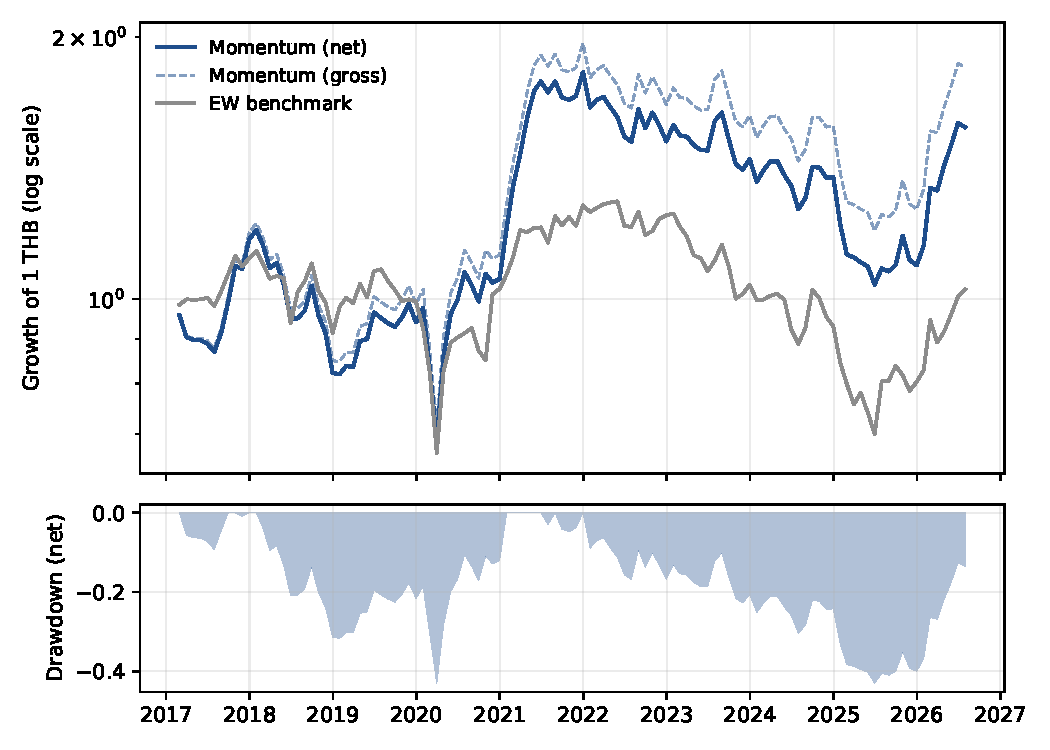
\includegraphics[width=\textwidth]{figures/equity_curve.pdf}
\caption{Growth of 1~THB invested in the momentum strategy (net and gross
of costs) and in the equal-weight benchmark of the same point-in-time
universe. Bottom panel: drawdown of the net strategy.}
\label{fig:equity}
\end{figure}

Table~\ref{tab:main} and Figure~\ref{fig:equity} summarize the study's
answer. The momentum portfolio earns 6.67\% per year gross and 4.90\% net,
against 0.28\% for the equal-weight benchmark --- a decade in which the
Thai market as a whole went essentially nowhere. The net active return of
3.73\% per year is economically meaningful in a flat market, and the
long-only strategy's maximum drawdown (43\%) is slightly \emph{shallower}
than the benchmark's (46\%).

%% TODO: เขียนย่อหน้าตีความเพิ่มด้วยคำพูดตัวเอง
Statistical significance, however, is weak. The active-return $t$-statistic
is 0.98; the gross top-minus-bottom spread --- the purest measure of the
signal --- earns 8.49\% per year with $t = 1.32$. At this sample length a
true annual edge of 3--4\% with 20\% tracking volatility is simply not
detectable at conventional thresholds: the study cannot distinguish skill
from luck, and says so.

\begin{table}[t]
\centering
\caption{Sub-period performance (net of costs).}
\label{tab:subperiods}
\begin{tabular}{lrrrr}
\toprule
Period & Months & Net CAGR & Benchmark CAGR & Active $t$ \\
\midrule
2016--2019 & 35 & -2.09\% & -0.25\% & -0.21 \\
2020--2022 & 36 & 17.30\% & 7.94\% & 0.76 \\
2023--2026 & 43 & 1.06\% & -5.31\% & 1.00 \\
\bottomrule
\end{tabular}

\end{table}

Table~\ref{tab:subperiods} shows the effect is regime-dependent. Nearly all
outperformance is earned in 2020--2022 (net 17.3\% vs.\ benchmark 7.9\%);
momentum lagged in the 2017--2019 sideways market, and in the 2023--2026
bear market it lost only 1\% while the benchmark lost 5.3\% per year ---
relative strength in a falling market, consistent with momentum's tendency
to load on whatever has been working, including defensive names in
downtrends.

\begin{table}[t]
\centering
\caption{Cost sensitivity of the momentum portfolio.}
\label{tab:costs}
\begin{tabular}{lrr}
\toprule
Cost per side & Net CAGR & Net Sharpe \\
\midrule
0.15\% & 5.60\% & 0.36 \\
0.25\% & 4.90\% & 0.33 \\
0.40\% & 3.86\% & 0.28 \\
\bottomrule
\end{tabular}

\end{table}

Table~\ref{tab:costs} shows the result is not an artifact of the cost
assumption: even at a punitive 0.40\% per side the strategy retains a
3.86\% net CAGR. The cost drag matters --- 56\% monthly turnover converts
a 0.40 gross Sharpe into 0.33 net --- but does not reverse the sign.

\section{Limitations}
\label{sec:limitations}
%% TODO: เรียงลำดับตามที่คิดว่าสำคัญสุดเอง
Six limitations qualify these results. (1)~Thirteen former members have no
recoverable price history; several (STARK, EARTH, IFEC) collapsed amid
fraud or default, and such names can carry high momentum ranks
\emph{before} collapsing, so their absence likely flatters the strategy ---
though takeover delistings (GLOW, DTAC, INTUCH), which typically end at a
premium, are missing too, partially offsetting the direction of the bias.
(2)~Restructuring gaps (SCB, GULF, STECON, TIDLOR) shorten several
important names' samples. (3)~The equal-weight benchmark is not the
capitalization-weighted SET100 index; it is the correct like-for-like
comparison for the strategy but understates what a passive index investor
earned in large-caps. (4)~Turnover ignores intra-month drift and the cost
model excludes market impact. (5)~Delisting-month returns are unobservable
in the data; positions are excluded at formation if the next month's return
is missing. (6)~One decade, one market: the sample is too short for the
$t$-statistics to settle the question, and no claim of external validity is
made.

\section{Future work}
%% TODO: ตัด/เพิ่มตามที่อยากทำจริง
Natural extensions, each to be pre-registered before estimation: recovering
delisting returns and terminal prices from SET's delisting statistics to
close the largest bias; cross-checking Yahoo prices against a second source
(e.g.\ Bloomberg) for the flagged names; quintile and 6-1 signal variants;
a volatility-managed overlay given the 43\% drawdown; and extending the
membership table back to 2005 using the same official documents, tripling
the sample length. A short leg is deliberately out of scope: securities
borrowing in Thailand is restricted to a subset of names with meaningful
fees, making the long-only formulation the realistic one.

\vspace{1em}
\noindent\textit{Tooling note.} The data pipeline, backtest engine and this
document's tables were built by the author with AI-assisted development
tools; all research design decisions, hypotheses and interpretations are
the author's own, and every number in this paper regenerates from the
public repository with two commands.

\bibliographystyle{plainnat}
\bibliography{references}

\appendix

\section{Membership coverage gaps}
\label{app:gaps}
The following symbols' price data falls short of their membership window
(generated by \texttt{scripts/make\_paper\_assets.py}).

\IfFileExists{tables/coverage_gaps.tex}{%
\begin{center}\small\begin{tabular}{lllll}
\toprule
Symbol & Data symbol & Member from & Data from & Status \\
\midrule
AWC & AWC & 2019-07 & 2019-10 & late start (+101d) \\
SCGP & SCGP & 2020-07 & 2020-10 & late start (+113d) \\
TIDLOR & TIDLOR & 2022-01 & 2025-05 & late start (+1231d) \\
PSH & PSH & 2016-07 & 2016-12 & late start (+153d) \\
GULF & GULF & 2019-01 & 2025-04 & late start (+2284d) \\
SCB & SCB & 2016-01 & 2022-04 & late start (+2301d) \\
STEC & STECON & 2016-01 & 2024-10 & late start (+3225d) \\
PS & PSH & 2016-01 & 2016-12 & late start (+335d) \\
SVI & SVI & 2016-01 & 2026-05 & late start (+3793d) \\
OR & OR & 2021-01 & 2021-02 & late start (+41d) \\
CRC & CRC & 2020-01 & 2020-02 & late start (+50d) \\
BSRC & BSRC & 2024-01 & -- & no data \\
DTAC & DTAC & 2016-01 & -- & no data \\
EARTH & EARTH & 2016-01 & -- & no data \\
ESSO & ESSO & 2018-01 & -- & no data \\
GL & GL & 2016-01 & -- & no data \\
GLOW & GLOW & 2016-01 & -- & no data \\
GOLD & GOLD & 2019-01 & -- & no data \\
IFEC & IFEC & 2016-07 & -- & no data \\
INTUCH & INTUCH & 2016-01 & -- & no data \\
KEX & KEX & 2022-01 & -- & no data \\
ROBINS & ROBINS & 2016-01 & -- & no data \\
SABUY & SABUY & 2023-01 & -- & no data \\
STARK & STARK & 2022-01 & -- & no data \\
\bottomrule
\end{tabular}
\end{center}
}{\textit{Run \texttt{python scripts/make\_paper\_assets.py} with the local
warehouse present to generate this table.}}

\section{Experiment registry}
\label{app:registry}
Every backtest executed against the data, in order, with no omissions.

\IfFileExists{tables/registry.tex}{%
\begin{center}\small\begin{tabular}{lllrrrl}
\toprule
Run & Signal & Top frac & Cost/side & Net CAGR & Net Sharpe & Note \\
\midrule
20260705-214914-208b2a & mom_12_1 & 0.1 & 0.25\% & 4.90\% & 0.33 & nan \\
\bottomrule
\end{tabular}
\end{center}
}{\textit{Generated from \texttt{research/experiments.csv} on the machine
holding the registry.}}

\end{document}
